\documentclass[10pt,fleq]{wlpeerj}
\usepackage{lmodern}
\usepackage{amssymb,amsmath}
\usepackage{ifxetex,ifluatex}
\usepackage{fixltx2e} % provides \textsubscript
\ifnum 0\ifxetex 1\fi\ifluatex 1\fi=0 % if pdftex
  \usepackage[T1]{fontenc}
  \usepackage[utf8]{inputenc}
\else % if luatex or xelatex
  \ifxetex
    \usepackage{mathspec}
  \else
    \usepackage{fontspec}
  \fi
  \defaultfontfeatures{Ligatures=TeX,Scale=MatchLowercase}
\fi
% use upquote if available, for straight quotes in verbatim environments
\IfFileExists{upquote.sty}{\usepackage{upquote}}{}
% use microtype if available
\IfFileExists{microtype.sty}{%
\usepackage{microtype}
\UseMicrotypeSet[protrusion]{basicmath} % disable protrusion for tt fonts
}{}
\usepackage[unicode=true]{hyperref}
\hypersetup{
            pdftitle={Format follows function: Agile editing of scientific manuscripts with markdown},
            pdfauthor={Robert Winkler},
            pdfkeywords={markdown,
latex,
publishing,
typesetting},
            pdfborder={0 0 0},
            breaklinks=true}
\urlstyle{same}  % don't use monospace font for urls
\usepackage{natbib}
\bibliographystyle{plainnat}
\usepackage{longtable,booktabs}
% Fix footnotes in tables (requires footnote package)
\IfFileExists{footnote.sty}{\usepackage{footnote}\makesavenoteenv{long table}}{}
\usepackage{graphicx,grffile}
\makeatletter
\def\maxwidth{\ifdim\Gin@nat@width>\linewidth\linewidth\else\Gin@nat@width\fi}
\def\maxheight{\ifdim\Gin@nat@height>\textheight\textheight\else\Gin@nat@height\fi}
\makeatother
% Scale images if necessary, so that they will not overflow the page
% margins by default, and it is still possible to overwrite the defaults
% using explicit options in \includegraphics[width, height, ...]{}
\setkeys{Gin}{width=\maxwidth,height=\maxheight,keepaspectratio}
\IfFileExists{parskip.sty}{%
\usepackage{parskip}
}{% else
\setlength{\parindent}{0pt}
\setlength{\parskip}{6pt plus 2pt minus 1pt}
}
\setlength{\emergencystretch}{3em}  % prevent overfull lines
\providecommand{\tightlist}{%
  \setlength{\itemsep}{0pt}\setlength{\parskip}{0pt}}
\setcounter{secnumdepth}{0}
% Redefines (sub)paragraphs to behave more like sections
\ifx\paragraph\undefined\else
\let\oldparagraph\paragraph
\renewcommand{\paragraph}[1]{\oldparagraph{#1}\mbox{}}
\fi
\ifx\subparagraph\undefined\else
\let\oldsubparagraph\subparagraph
\renewcommand{\subparagraph}[1]{\oldsubparagraph{#1}\mbox{}}
\fi

% set default figure placement to htbp
\makeatletter
\def\fps@figure{htbp}
\makeatother


\title{Format
follows
function:
Agile
editing of
scientific
manuscripts
with
markdown}
\author{Robert
Winkler}
\date{}

\begin{document}
\maketitle
\begin{abstract}
Publishing
is an
essential
part of
academic
life. The
material
for books,
seminar
lectures
and
journal
manuscripts
has to be
prepared
in
specific
formats.
Scientific
manuscripts
consist of
contents,
including
text,
figures,
formulas,
tables and
citations,
which are
presented
in a
certain
format.
This
format
depends on
the
intended
use,
e.g.~for
for
submission
to a
particular
journal,
publication
as a
printed or
electronic
book, or
for a
webpage.
Incompatible
file
formats,
markdown
with
different
target
formats.
This
article
demonstrates
the
feasability
to edit
the
contents
for
various
academic
pubication
formats in
a common
format.
Markdown
files
containing
the
content
with some
simple
formatting
rules in
plain
text,
which
facilitates
the
writing.
The final
document
can be
exported
to
high-quality
publications
in
different
formats
using
Pandoc.
\end{abstract}

\textbf{Correspondence}:
robert.winkler@cinvestav.mx,
CINVESTAV
Unidad
Irapuato,
Department
of
Biochemistry
and
Biotechnology,
Laboratory
of
Biochemical
and
Instrumental
Analysis
(labABI,
\url{http://www.ira.cinvestav.mx/lababi.aspx}),
Km. 9.6
Libramiento
Norte
Carr.
Irapuato-León
36821
Irapuato,
Gto.
Mexico,
Tel.: +52
(462) 623
96 35, Fax
+52 (462)
624 58 46

\textbf{Keywords}:
markdown,
latex,
publishing,
typesetting

\section{Introduction}\label{introduction}

Even if a
submitted
manuscript
might be
accepted
by a
journal
`as is',
it still
needs to
be
adjusted
to the
particular
publication
style in
the
production
stage.
Generally
speaking,
a
scientific
manuscript
is
composed
from
contents
and
formatting.
Whilst the
content,
i.e.~text,
figures,
tables,
citations
etc., may
remain the
same
between
different
publishing
forms and
journal
styles,
the
formatting
can be
rather
different.
Current
publishing
formats
PDF HTML
EPUB.
Typesetting
software,
word
processors
such as
Microsoft
Word,
LibreOffice,
WPS
Office,
What You
See Is
What You
Get
(WYSIWYG),
LaTeX What
You See Is
What You
Want
(WYSIWYW),
hybrids
such as
LyX What
You See Is
What You
Mean
(WYSIWYM).
Because of
the
sometimes
complicated
syntax
specifications,
simple
conversions
between
file
formats
can be
difficult
or
impossible.
In
academic
publishing,
the
following
types of
works
require
the
creation
of
different
output
formats
from the
same
source
text:

\begin{itemize}
\tightlist
\item
  For the
  publishing
  of a
  book,
  with a
  print
  version
  in PDF
  and an
  electronic
  version
  in EPUB.
\item
  For
  distributing
  of a
  seminar
  script,
  with an
  online
  version
  in HTML
  and a
  print
  version
  in PDF.
\item
  For
  submitting
  a
  journal
  manuscript
  for
  peer-review
  in DOCX,
  as well
  as a
  pre-print
  version
  with
  another
  journal
  style in
  PDF.
\end{itemize}

\subsection{Comparison
of
different
markup
languages}\label{comparison-of-different-markup-languages}

\textbf{Table
1.}
Formatting
elements
and their
implementation
in
different
document
types.

\begin{longtable}[]{@{}llll@{}}
\toprule
\begin{minipage}[b]{0.24\columnwidth}\raggedright\strut
Element\strut
\end{minipage}
&
\begin{minipage}[b]{0.15\columnwidth}\raggedright\strut
Markdown\strut
\end{minipage}
&
\begin{minipage}[b]{0.26\columnwidth}\raggedright\strut
LaTeX\strut
\end{minipage}
&
\begin{minipage}[b]{0.24\columnwidth}\raggedright\strut
HTML\strut
\end{minipage}\tabularnewline
\midrule
\endhead
\begin{minipage}[t]{0.24\columnwidth}\raggedright\strut
\textbf{structure}\strut
\end{minipage}
&
\begin{minipage}[t]{0.15\columnwidth}\raggedright\strut
\strut
\end{minipage}
&
\begin{minipage}[t]{0.26\columnwidth}\raggedright\strut
\strut
\end{minipage}
&
\begin{minipage}[t]{0.24\columnwidth}\raggedright\strut
\strut
\end{minipage}\tabularnewline
\begin{minipage}[t]{0.24\columnwidth}\raggedright\strut
section\strut
\end{minipage}
&
\begin{minipage}[t]{0.15\columnwidth}\raggedright\strut
\texttt{\#\ Intro}\strut
\end{minipage}
&
\begin{minipage}[t]{0.26\columnwidth}\raggedright\strut
\texttt{\textbackslash{}section\{Intro\}}\strut
\end{minipage}
&
\begin{minipage}[t]{0.24\columnwidth}\raggedright\strut
\texttt{\textless{}h1\textgreater{}\textless{}Intro\textgreater{}\textless{}/h1\textgreater{}}\strut
\end{minipage}\tabularnewline
\begin{minipage}[t]{0.24\columnwidth}\raggedright\strut
subsection\strut
\end{minipage}
&
\begin{minipage}[t]{0.15\columnwidth}\raggedright\strut
\texttt{\#\#\ History}\strut
\end{minipage}
&
\begin{minipage}[t]{0.26\columnwidth}\raggedright\strut
\texttt{\textbackslash{}subsection\{History\}}\strut
\end{minipage}
&
\begin{minipage}[t]{0.24\columnwidth}\raggedright\strut
\texttt{\textless{}h2\textgreater{}\textless{}History\textgreater{}\textless{}/h2\textgreater{}}\strut
\end{minipage}\tabularnewline
\begin{minipage}[t]{0.24\columnwidth}\raggedright\strut
\textbf{text
formatting}\strut
\end{minipage}
&
\begin{minipage}[t]{0.15\columnwidth}\raggedright\strut
\strut
\end{minipage}
&
\begin{minipage}[t]{0.26\columnwidth}\raggedright\strut
\strut
\end{minipage}
&
\begin{minipage}[t]{0.24\columnwidth}\raggedright\strut
\strut
\end{minipage}\tabularnewline
\begin{minipage}[t]{0.24\columnwidth}\raggedright\strut
bold\strut
\end{minipage}
&
\begin{minipage}[t]{0.15\columnwidth}\raggedright\strut
\texttt{**text**}\strut
\end{minipage}
&
\begin{minipage}[t]{0.26\columnwidth}\raggedright\strut
\texttt{\textbackslash{}textbf\{text\}}\strut
\end{minipage}
&
\begin{minipage}[t]{0.24\columnwidth}\raggedright\strut
\texttt{text}\strut
\end{minipage}\tabularnewline
\begin{minipage}[t]{0.24\columnwidth}\raggedright\strut
\textbf{cross
references}\strut
\end{minipage}
&
\begin{minipage}[t]{0.15\columnwidth}\raggedright\strut
\strut
\end{minipage}
&
\begin{minipage}[t]{0.26\columnwidth}\raggedright\strut
\strut
\end{minipage}
&
\begin{minipage}[t]{0.24\columnwidth}\raggedright\strut
\strut
\end{minipage}\tabularnewline
\begin{minipage}[t]{0.24\columnwidth}\raggedright\strut
to
section\strut
\end{minipage}
&
\begin{minipage}[t]{0.15\columnwidth}\raggedright\strut
\strut
\end{minipage}
&
\begin{minipage}[t]{0.26\columnwidth}\raggedright\strut
\strut
\end{minipage}
&
\begin{minipage}[t]{0.24\columnwidth}\raggedright\strut
\texttt{text}\strut
\end{minipage}\tabularnewline
\begin{minipage}[t]{0.24\columnwidth}\raggedright\strut
http
link\strut
\end{minipage}
&
\begin{minipage}[t]{0.15\columnwidth}\raggedright\strut
\strut
\end{minipage}
&
\begin{minipage}[t]{0.26\columnwidth}\raggedright\strut
\strut
\end{minipage}
&
\begin{minipage}[t]{0.24\columnwidth}\raggedright\strut
\texttt{text}\strut
\end{minipage}\tabularnewline
\bottomrule
\end{longtable}

Documents
with the
commonly
used
Office
Open XML
(DOCX
Microsoft
Word
files) and
OpenDocument
(ODT
LibreOffice)
file
formats
can be
opened in
a standard
text
editor
after
unzipping.
However,
content
and
formatting
information
is
distributed
into
various
folders
and
files.\\
Overall,
markdown
displays
the
simplest
structure,
which
facilitates
the
editing of
documents.

\section{Concepts
of
markdown
and
Pandoc}\label{concepts-of-markdown-and-pandoc}

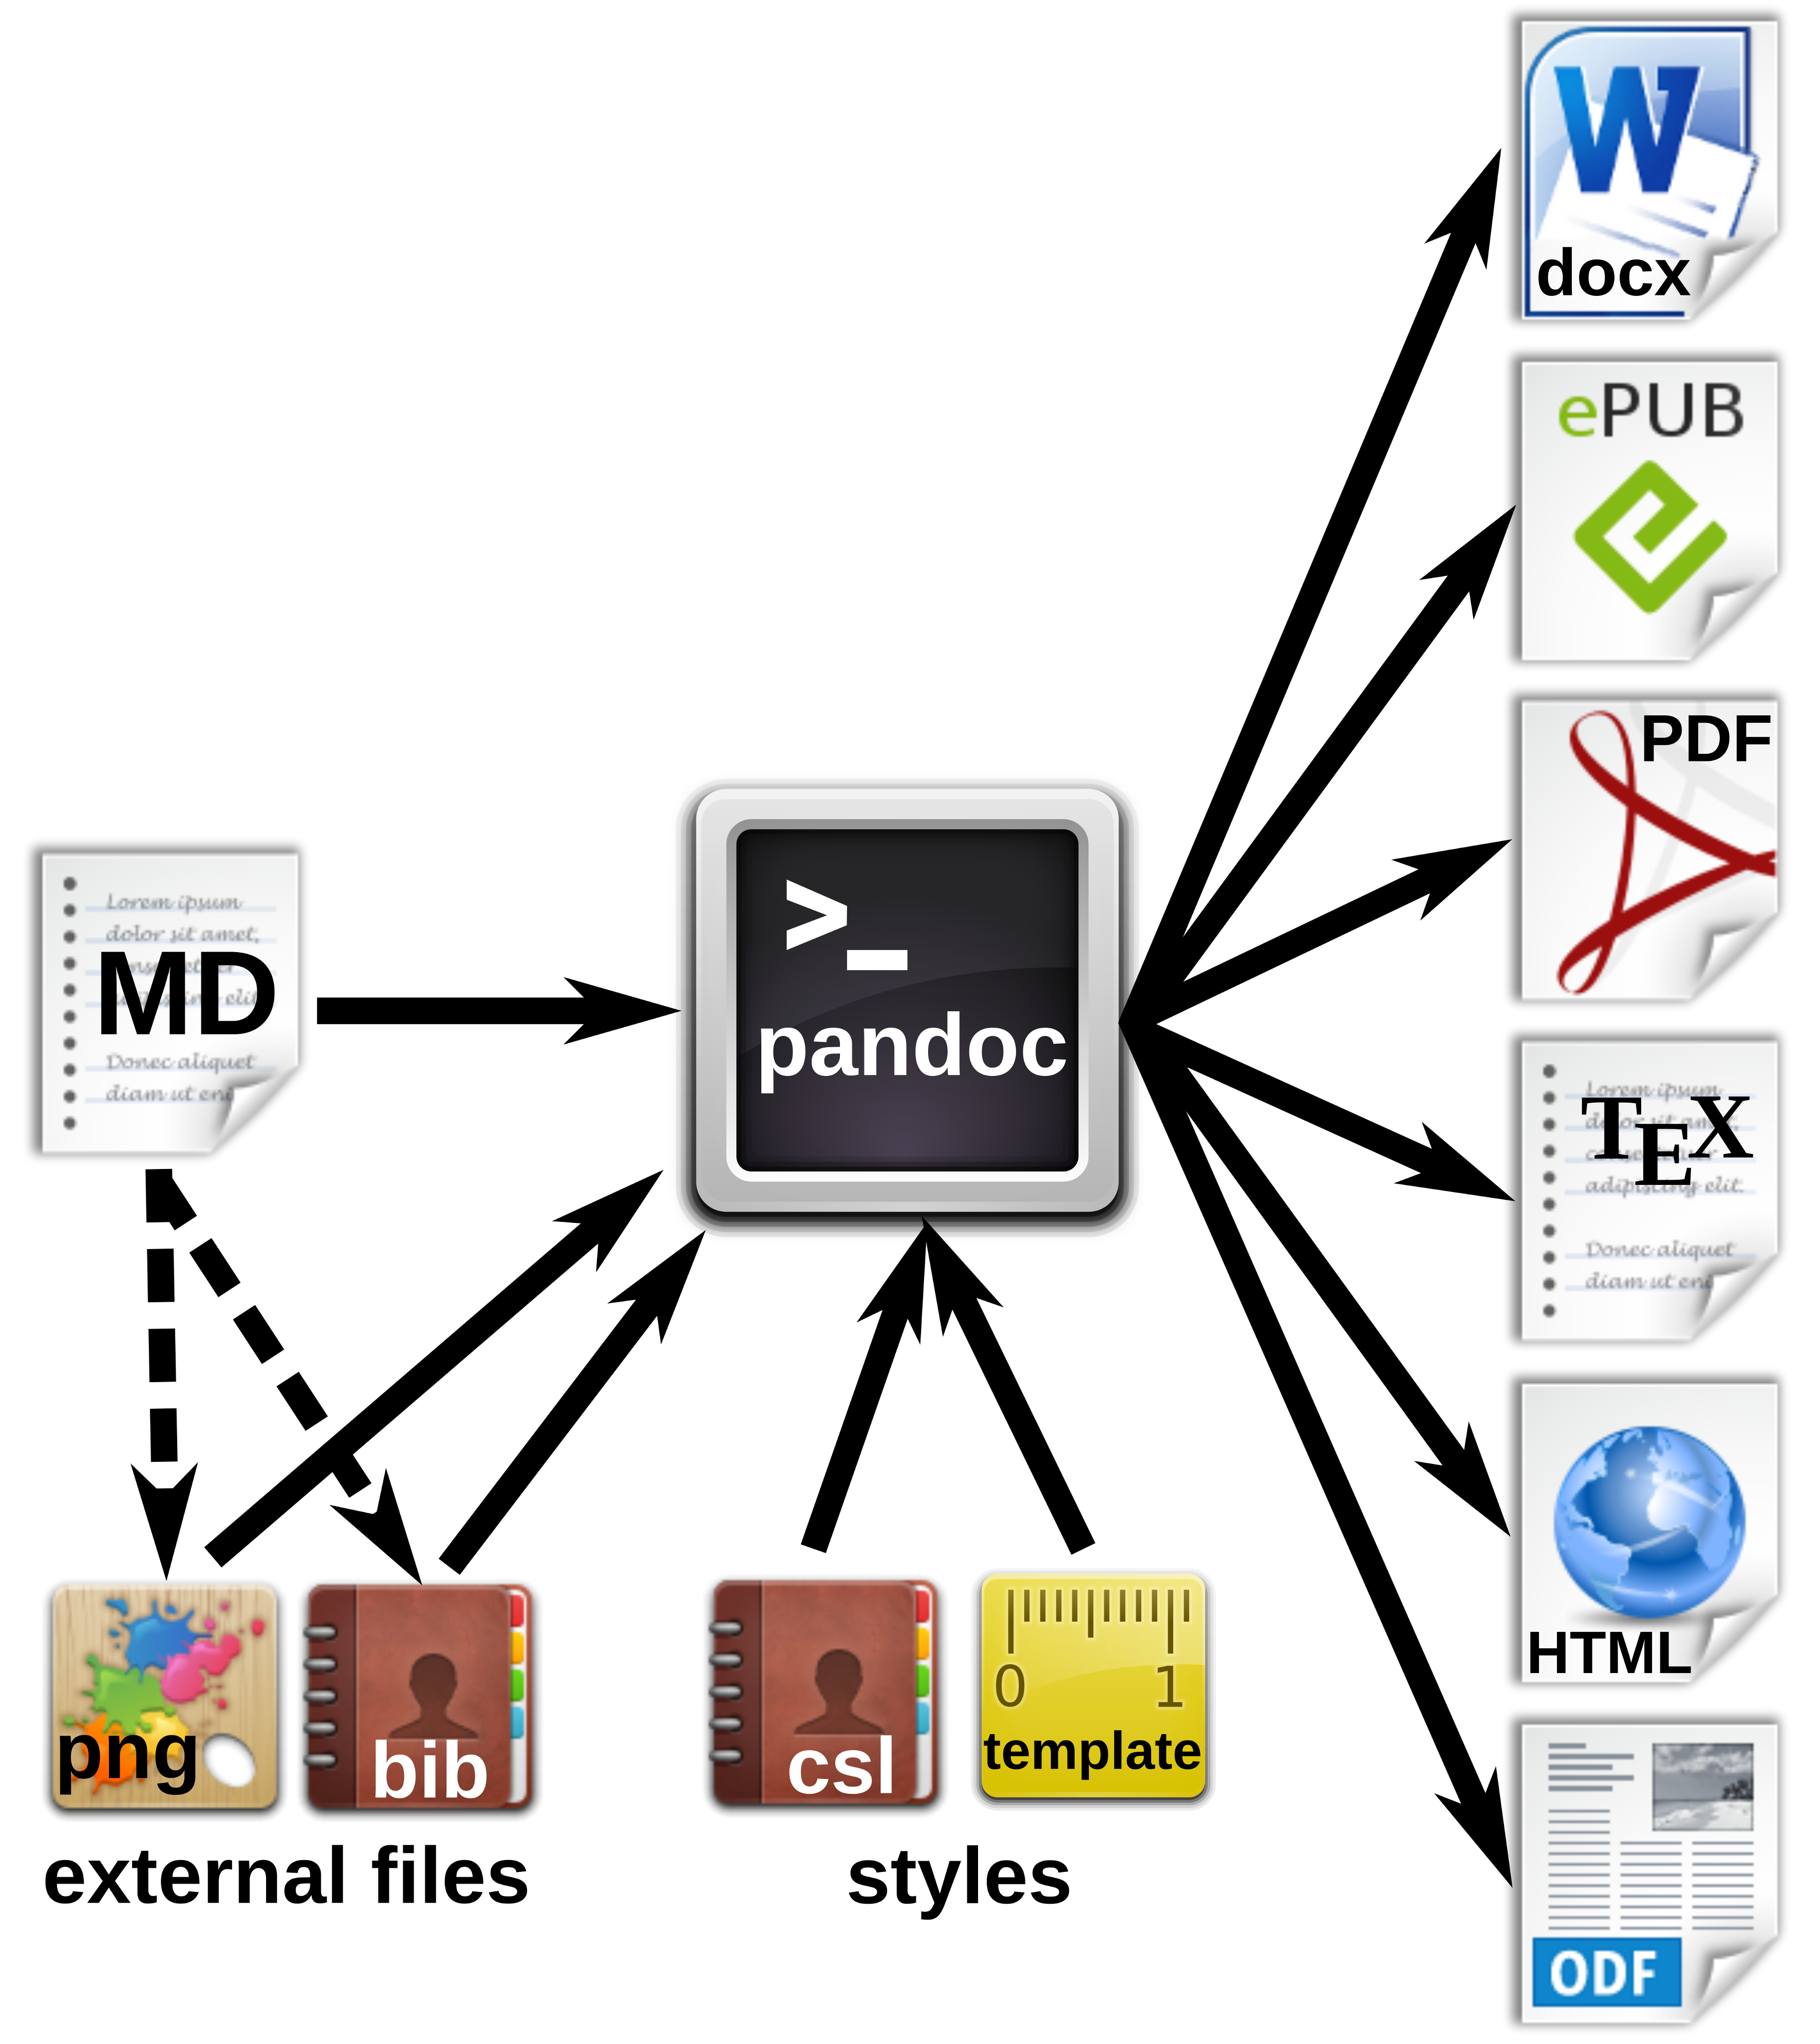
\includegraphics{fig-pandoc-workflow.png}
\textbf{Figure
xx.}
Workfow
for the
generation
of
multiple
document
formats
with
Pandoc.

\section{Markdown
editors
and online
editing}\label{markdown-editors-and-online-editing}

\subsection{Editing
programs}\label{editing-programs}

Because of
the simple
syntax,
basically
any text
editor is
suitable
for
editing
markdown
files. For
several
popular
text
editors,
such as
vim
(\url{http://www.vim.org/}),
GNU Emacs
(\url{https://www.gnu.org/software/emacs/}),
atom
(\url{https://atom.io/})
or geany
(\url{http://www.geany.org/}),
plugins
provide
additional
functionality
for
markdown
editing,
such as
syntax
highlighting,
live
preview or
structure
browsing.\\
On the
other
side, in
the last
years
plenty of
special
mardown
editors
have been
published.
Many of
those are
cross-platform
compatible,
e.g.~Abricotine
(\url{http://abricotine.brrd.fr/}),
Ghostview
(\url{https://github.com/wereturtle/ghostwriter})
and
CuteMarkEd
(\url{https://cloose.github.io/CuteMarkEd/}).\\
xx Writing
on the go
mobile
devices,
Even for
tablets,
Android
and iOS
devices,
numerous
free and
low-cost
applications
exist.
Parts of
this text
were
written in
xx
JotterPad
dictation
and swipe
softwarexx
Various of
those
applications
support
the cloud
storage of
documents.

\textbf{Figure
xx.}
Coding,
preview
and table
of
contents
view using
the
CuteMarkEd
editor.

\subsection{Online
editing
and
collaborative
writing}\label{online-editing-and-collaborative-writing}

xx Google
Docs test
editing.

In recent
years,
several
platforms
were
developed
for
collaborative
writing.
Google
Docs.
OwnCloud
with
Markdown
Editor
plugin
(see
section
xx).

\textbf{Figure
2.} Direct
online
editing of
this
manuscript
with live
preview
using the
ownCloud
Markdown
Editor
plugin by
Robin
Appelman.

\subsection{Document
versioning
and change
control}\label{document-versioning-and-change-control}

Integrated
in editing
software
or cloud
server,
low
overhead
of the
files
diff, git.

\section{Pandoc
markdown
for
scientific
texts}\label{pandoc-markdown-for-scientific-texts}

\subsection{Tables}\label{tables}

Pipe
tables are
less
strict in
their
syntax

\begin{verbatim}
| Left | Center | Right | Default |
|:-----|:------:|------:|---------|
| LLL  | CCC    | RRR   | DDD     |
\end{verbatim}

gives

\begin{longtable}[]{@{}lcrl@{}}
\toprule
\begin{minipage}[b]{0.17\columnwidth}\raggedright\strut
Left\strut
\end{minipage}
&
\begin{minipage}[b]{0.24\columnwidth}\centering\strut
Center\strut
\end{minipage}
&
\begin{minipage}[b]{0.20\columnwidth}\raggedleft\strut
Right\strut
\end{minipage}
&
\begin{minipage}[b]{0.27\columnwidth}\raggedright\strut
Default\strut
\end{minipage}\tabularnewline
\midrule
\endhead
\begin{minipage}[t]{0.17\columnwidth}\raggedright\strut
LLL\strut
\end{minipage}
&
\begin{minipage}[t]{0.24\columnwidth}\centering\strut
CCC\strut
\end{minipage}
&
\begin{minipage}[t]{0.20\columnwidth}\raggedleft\strut
RRR\strut
\end{minipage}
&
\begin{minipage}[t]{0.27\columnwidth}\raggedright\strut
DDD\strut
\end{minipage}\tabularnewline
\bottomrule
\end{longtable}

\subsection{Figures}\label{figures}

\subsection{Formula}\label{formula}

Formula
can be
inserted
in LaTeX
mode using
delimiters
(\texttt{\$}
for
Pandoc,
\texttt{\$\$}
adds
compatibility
for online
preview
rendering
with
CuteMarkEd/MathJax).
E.g. the
formula
for
calculating
the
standard
deviation
\(s\) of a
random
sampling
would be
written
as:

\begin{verbatim}
$s=\sqrt{\frac{1}{N-1}\sum_{i=1}^N(x_i-\overline{x})^{2}}$
\end{verbatim}

and gives:

\(s=\sqrt{\frac{1}{N-1}\sum_{i=1}^N(x_i-\overline{x})^{2}}\)

with
\(x_i\)
the
individual
observations,
\(\overline{x}\)
the sample
mean and
\(N\) the
total
number of
samples.

\subsection{Code
listings}\label{code-listings}

\section{Citations
and
biography}\label{citations-and-biography}

\subsection{Reference
databases}\label{reference-databases}

bibtex
databases,
which are
supported
by almost
any
reference
management
program.

\subsection{Database
of cited
references}\label{database-of-cited-references}

A bibtex
data base
for the
cited
references
only using
BibTool:

\begin{enumerate}
\def\labelenumi{\arabic{enumi}.}
\tightlist
\item
  Extract
  refrence
  keys.
  This can
  be done
  by a
  simple
  Perl
  (\url{https://www.perl.org/})
  command:
  \textsubscript{\textasciitilde{}}
  perl -ne
  `print
  ``\$1,''
  if
  /(?\textless{}=@)(.+?)(?={[}{]},{]})/'
  agile-editing-pandoc.md
  \textsubscript{\textasciitilde{}}
  The
  command
  prints
  out the
  keys of
  the file
  \texttt{agile-editing-pandoc.md},
  separated
  by
  comas.
  The
  domains
  of email
  adresses
  also
  will be
  returned,
  but this
  does not
  affect
  the
  creation
  of the
  final
  database.
\item
  Write an
  bibtex
  \texttt{.aux}
  file
  (e.g.
  \texttt{bibextract.aux})
  containing
  the name
  of the
  database
  (here:
  \texttt{zotero.bib})
  and the
  extracted
  keys,
  separated
  by comas
  (from
  the
  previous
  step):
  \textsubscript{\textsubscript{\textsubscript{
  \bibstyle{alpha}
  \bibdata{zotero.bib}
  \citation{smith_software_2016,key2,key3}
  }}}
\item
  Process
  the
  complete
  database
  to
  extract
  the
  cited
  references
  into a
  now
  database
  (called
  \texttt{bibshort.bib}):
  \textsubscript{\textasciitilde{}}
  bibtool
  -x
  bibextract.aux
  -o
  bibshort.bib
  \textsubscript{\textasciitilde{}}
\end{enumerate}

\subsection{Styles}\label{styles}

Whereas
natbib
bibtex is
supported
by Pandoc,
it is
incompatible
with DOCX
xx. The
Citation
Style
Language
(CSL)
\url{http://citationstyles.org/}
is used
for the
citations
and
bibliographies.
This file
format is
supported
e.g.~by
the
reference
management
programs
Mendeley
\url{https://www.mendeley.com/},
Papers
\url{http://papersapp.com/}
and Zotero
\url{https://www.zotero.org/}.\\
CSL styles
for
particular
journals
can be
found from
the Zotero
style
repository
\url{https://www.zotero.org/styles}.\\
The
bibliography
style,
which
Pandoc
should use
for the
target
document
can be
chosen or
in the
YAML block
of the
markdown
document
or can be
passed as
an command
line
option.
The later
is more
recommendable,
because
different
bibliography
style may
be used
for
different
documents.

\subsection{Creation
of natbib
citations
in
LaTeX}\label{creation-of-natbib-citations-in-latex}

For
citations
in
scientific
manuscripts
written in
LaTex, the
natbib
package is
widely
used. To
create TEX
output
file with
natbib
citations,
Pandoc
simply has
to be run
with the
\texttt{-\/-natbib}
option.

\section{Document
code and
software
availability}\label{document-code-and-software-availability}

The
software
used was
cited
according
to
\citep[p23]{smith_software_2016, winkler_esiprot:_2010}.
Since
unique
identifiers
are
missing
for most
software
projects,
we only
refer to
the
project
homepages
or
software
repositories:

\begin{longtable}[]{@{}llllll@{}}
\toprule
\begin{minipage}[b]{0.09\columnwidth}\raggedright\strut
Software\strut
\end{minipage}
&
\begin{minipage}[b]{0.20\columnwidth}\raggedright\strut
Use\strut
\end{minipage}
&
\begin{minipage}[b]{0.17\columnwidth}\raggedright\strut
Authors\strut
\end{minipage}
&
\begin{minipage}[b]{0.05\columnwidth}\raggedright\strut
Version\strut
\end{minipage}
&
\begin{minipage}[b]{0.07\columnwidth}\raggedright\strut
Release
date\strut
\end{minipage}
&
\begin{minipage}[b]{0.26\columnwidth}\raggedright\strut
Homepage/
repository\strut
\end{minipage}\tabularnewline
\midrule
\endhead
\begin{minipage}[t]{0.09\columnwidth}\raggedright\strut
Pandoc\strut
\end{minipage}
&
\begin{minipage}[t]{0.20\columnwidth}\raggedright\strut
universal
markup
converter\strut
\end{minipage}
&
\begin{minipage}[t]{0.17\columnwidth}\raggedright\strut
John
MacFarlane\strut
\end{minipage}
&
\begin{minipage}[t]{0.05\columnwidth}\raggedright\strut
1.16.0.2\strut
\end{minipage}
&
\begin{minipage}[t]{0.07\columnwidth}\raggedright\strut
2016/01/13\strut
\end{minipage}
&
\begin{minipage}[t]{0.26\columnwidth}\raggedright\strut
\url{http://www.pandoc.org}\strut
\end{minipage}\tabularnewline
\begin{minipage}[t]{0.09\columnwidth}\raggedright\strut
pandoc-citeproc\strut
\end{minipage}
&
\begin{minipage}[t]{0.20\columnwidth}\raggedright\strut
library
for CSL
citations
with
Pandoc\strut
\end{minipage}
&
\begin{minipage}[t]{0.17\columnwidth}\raggedright\strut
John
MacFarlane,
Andrea
Rossato\strut
\end{minipage}
&
\begin{minipage}[t]{0.05\columnwidth}\raggedright\strut
0.9.1\strut
\end{minipage}
&
\begin{minipage}[t]{0.07\columnwidth}\raggedright\strut
2016/03/19\strut
\end{minipage}
&
\begin{minipage}[t]{0.26\columnwidth}\raggedright\strut
\url{https://github.com/jgm/pandoc-citeproc}\strut
\end{minipage}\tabularnewline
\begin{minipage}[t]{0.09\columnwidth}\raggedright\strut
ownCloud\strut
\end{minipage}
&
\begin{minipage}[t]{0.20\columnwidth}\raggedright\strut
personal
cloud
software\strut
\end{minipage}
&
\begin{minipage}[t]{0.17\columnwidth}\raggedright\strut
ownCloud
GmbH,
Community\strut
\end{minipage}
&
\begin{minipage}[t]{0.05\columnwidth}\raggedright\strut
9.1.1\strut
\end{minipage}
&
\begin{minipage}[t]{0.07\columnwidth}\raggedright\strut
2016/09/20\strut
\end{minipage}
&
\begin{minipage}[t]{0.26\columnwidth}\raggedright\strut
\url{https://owncloud.org/}\strut
\end{minipage}\tabularnewline
\begin{minipage}[t]{0.09\columnwidth}\raggedright\strut
Markdown
Editor\strut
\end{minipage}
&
\begin{minipage}[t]{0.20\columnwidth}\raggedright\strut
plugin for
ownCloud\strut
\end{minipage}
&
\begin{minipage}[t]{0.17\columnwidth}\raggedright\strut
Robin
Appelman\strut
\end{minipage}
&
\begin{minipage}[t]{0.05\columnwidth}\raggedright\strut
0.1\strut
\end{minipage}
&
\begin{minipage}[t]{0.07\columnwidth}\raggedright\strut
2016/03/08\strut
\end{minipage}
&
\begin{minipage}[t]{0.26\columnwidth}\raggedright\strut
\url{https://github.com/icewind1991/files_markdown}\strut
\end{minipage}\tabularnewline
\begin{minipage}[t]{0.09\columnwidth}\raggedright\strut
BibTool\strut
\end{minipage}
&
\begin{minipage}[t]{0.20\columnwidth}\raggedright\strut
Bibtex
database
tool\strut
\end{minipage}
&
\begin{minipage}[t]{0.17\columnwidth}\raggedright\strut
Gerd
Neugebauer\strut
\end{minipage}
&
\begin{minipage}[t]{0.05\columnwidth}\raggedright\strut
2.63\strut
\end{minipage}
&
\begin{minipage}[t]{0.07\columnwidth}\raggedright\strut
2016/01/16\strut
\end{minipage}
&
\begin{minipage}[t]{0.26\columnwidth}\raggedright\strut
\url{https://github.com/ge-ne/bibtool}\strut
\end{minipage}\tabularnewline
\bottomrule
\end{longtable}

xx
CuteMarkEd
xx xx
JotterPad
Prof xx
Pandoc is
available
for
Windows,
Mac OS X,
Linux, BSD
and as
source
code.

The source
code of
this
manuscript,
as well as
templates
and the
Pandoc
script
have been
deposited
to xx.

\section{Definition
of output
formatting}\label{definition-of-output-formatting}

command
line
parameters
and
templates
xx

\section{Example:
Manuscript
with
output of
DOCX
format and
TEX/PDF
for PeerJ
pre-print
submission}\label{example-manuscript-with-output-of-docx-format-and-texpdf-for-peerj-pre-print-submission}

\subsection{Development
of DOCX
template}\label{development-of-docx-template}

A first
DOCX
document
with
bibliography
in APA
format is
created
with
Pandoc
DOCX
output:

\begin{verbatim}
pandoc -S -s --csl=apa.csl --filter pandoc-citeproc
-o pandoc-manuscript.docx agile-editing-pandoc.md
\end{verbatim}

The
document
settings
and styles
of the
resulting
file
\texttt{pandoc-manuscript.docx}
can be
modified,
and
following
it can be
used as
document
template
(\texttt{-\/-reference-docx=pandoc-manuscript.docx}).

\begin{verbatim}
pandoc -S -s --reference-docx=pandoc-manuscript.docx
--csl=apa.csl --filter pandoc-citeproc -o outfile.docx agile-editing-pandoc.md
\end{verbatim}

It is
possible
to
directly
re-use a
previous
output
file as
template
(i.e.~template
and output
file have
the same
file
name):

\begin{verbatim}
pandoc -S -s --columns=10 --reference-docx=outfile.docx --csl=apa.csl --filter pandoc-citeproc -o outfile.docx agile-editing-pandoc.md
\end{verbatim}

In this
way, the
template
can be
incrementally
adjusted
to the
desired
document
formatting.
The final
document
may be
employed
later as
Pandoc
template
for other
manuscripts
with the
same
specifications.
In this
case,
running
Pandoc the
first time
with the
template,
the
contents
of the new
manuscript
would be
filled
into the
provided
DOCX
template.
A page
with DOCX
manuscript
formatting
of this
article is
shown in
figure xx.

\textbf{Figure
xx.} DOCX
output
with a
modified
document
template.

\subsection{Development
of a
TEX/PDF
template}\label{development-of-a-texpdf-template}

\begin{verbatim}
pandoc -D latex > template-peerj.latex
\end{verbatim}

\section{Conclusions}\label{conclusions}

Writing
scientific
manuscripts
in
markdown
format
helps to
focus on
the
content
rather
than on
the
format.
Lightweight
format
facilitates
file
editing
and
handling.
With the
same
source
file,
multiple
output
files for
different
uses or
publisher's
specifications
c can be
generated
with
Pandoc.
Therefore,
a workflow
based on
markdown
format is
certainly
an
attractive
option for
scientific
writers.
Therefore,
scientific
publishers
should
consider
to support
the
submission
of
documents
in
markdown
format.

\section{Acknowledgments}\label{acknowledgments}

We
cordially
thank
Dr.~Gerd
Neugebauer
for his
help in
creating a
subset of
a bibtex
data base
using
BibTool.
The work
was funded
by the
Consejo
Nacional
de Ciencia
y
Tecnología
(CONACyT)
Mexico,
with the
grant
FRONTERAS
2015-2/814
and by
institutional
funding of
the Centro
de
Investigación
y de
Estudios
Avanzados
del
Instituto
Politécnico
Nacional
(CINVESTAV).

\renewcommand\refname{Bibliography}
\bibliography{zotero.bib}

\end{document}
